%----------------------------------------------------------------------------
\chapter{Kivitelezés}
%----------------------------------------------------------------------------


A megtervezett alkotás értékelése és kritikai elemzése.

Minden komponensre egy alfejezetet kell szánni, amelyben részletesen leírjuk a komponens belső működését, pl. osztálydiagramok segítségével.
Ha komponens más komponensekkel is kollaborál (igénybe veszi egy másik komponens publikus interface-ét vagy egy külső libraryt, függőséget/dependenciát használ), akkor ezt egy aktivitás-, vagy szekvencia diagrammal kell szemléltetni: pl. ki indítja a kommunikációt, mennyit vár, stb.


Ne próbáljunk egy diagrammal elintézni mindent. Érdemes egy használati esetre mint például a bejelentkezés vagy keresés egy-egy szekvencia diagramot készíteni. Annyi diagramot kell készíteni, amennyi elégséges ahhoz, hogy bemutassuk a rendszert. Figyelni kell, mert egyes diagramok a rendszer más-más aspektusait emelik ki (pl. Használati eset- és szekvencia diagram dinamikus képet, míg az osztálydiagram statikus képet ad a rendszerről).


Szoftverfejlesztés esetében ide lehet tenni a rendszerről készített képernyőképeket is. Lehet készíteni felhasználói útmutatót is. Érdemes csak a releváns részleteket bemutatni (nem releváns a bejelentkezés, releváns, hogy  mi történik a bejelentkezés után). A lényegesebb részeknél lehet konkrét kódrészletet is bemutatni. 





\section{P\'eld\'ak}

\begin{center}
	\begin{algorithm}[H]
		\KwIn{
			Integers $a \geq 0$ and $b \geq 0$}
		\KwOut{\textsc{Gcd} of $a$ and $b$} \While{$b \neq 0$}{
			$r \leftarrow a \bmod b$\;
			$a \leftarrow b$\;
			$b \leftarrow r$\;
		}
		\caption{Euclidean Algorithm}
	\end{algorithm}
\end{center}







\begin{algorithm}[H]
	\SetAlgoLined
	\KwData{this text}
	\KwResult{how to write algorithm with \LaTeX2e }
	initialization\;
	\While{not at end of this document}{
		read current\;
		\eIf{understand}{
			go to next section\;
			current section becomes this one\;
		}{
			go back to the beginning of current section\;
		}
	}
	\caption{How to write algorithms}
\end{algorithm}

\newpage
\begin{algorithm}[H]
	\DontPrintSemicolon
	\KwData{$G=(X,U)$ such that $G^{tc}$ is an order.}
	\KwResult{$G’=(X,V)$ with $V\subseteq U$ such that $G’^{tc}$ is an
		interval order.}
	\Begin{
		$V \longleftarrow U$\;
		$S \longleftarrow \emptyset$\;
		\For{$x\in X$}{
			$NbSuccInS(x) \longleftarrow 0$\;
			$NbPredInMin(x) \longleftarrow 0$\;
			$NbPredNotInMin(x) \longleftarrow |ImPred(x)|$\;
		}
		\For{$x \in X$}{
			\If{$NbPredInMin(x) = 0$ {\bf and} $NbPredNotInMin(x) = 0$}{
				$AppendToMin(x)$}
		}
		\nl\While{$S \neq \emptyset$}{\label{InRes1}
			\nlset{REM} remove $x$ from the list of $T$ of maximal index\;\label{InResR}
			\lnl{InRes2}\While{$|S \cap ImSucc(x)| \neq |S|$}{
				\For{$ y \in S-ImSucc(x)$}{
					\{ remove from $V$ all the arcs $zy$ : \}\;
					\For{$z \in ImPred(y) \cap Min$}{
						remove the arc $zy$ from $V$\;
						$NbSuccInS(z) \longleftarrow NbSuccInS(z) - 1$\;
						move $z$ in $T$ to the list preceding its present list\;
						\{i.e. If $z \in T[k]$, move $z$ from $T[k]$ to
						$T[k-1]$\}\;
					}
					$NbPredInMin(y) \longleftarrow 0$\;
					$NbPredNotInMin(y) \longleftarrow 0$\;
					$S \longleftarrow S - \{y\}$\;
					$AppendToMin(y)$\;
				}
			}
			$RemoveFromMin(x)$\;
		}
	}
	\caption{IntervalRestriction\label{IR}}
\end{algorithm}


Az általam írt szoftver egy \textbf{Java nyelv}en, \textbf{NetBeans IDE 8.0.1} fejlesztői környezetben írt asztali alkalmazás, amelynek fő funkcionalitása a kezdetiérték-probléma típusú differenciálegyenletek numerikus megoldása és ezen megoldások grafikus felületen való ábrázolása. A fő funkcionalitás mellett a szoftver tartalmaz még két kisebb funkcionalitást is, ezek közül az egyik a kétdimenziós függvényábrázolási lehetőség, a másik pedig a háromdimenziós függvények megjelenítésének lehetősége.

Az szoftver a differenciálegyenletek megoldásához a \ref{fejezet3}. fejezetben leírt numerikus eljárásokat alkalmazza.

A grafikus felhasználói felület megalkotásához a \textbf{Swing} (Java) komponens készletet használtam. A Swing használatával célom az volt, hogy egy felhasználóbarát és könnyen kezelhető felületet hozzak létre, amelyen a felhasználó könnyedén eligazodhat. Továbbá e komponenskészlet használata mellett szól az is, hogy a későbbiekben bemutatásra kerülő könyvtárak, melyek az ábrázolás megvalósítására használtam szintén Swing komponensekkel vannak megvalósítva.

Felhasználói felület, valamint a három funkcionalitás bemutatása képekben:

\begin{algorithm}[H]
	\Switch{order}{
		\uCase{bloody mary}{
			Add tomato juice\;
			Add vodka\;
			break\;
		}
		\uCase{hot whiskey}{
			Add whiskey\;
			Add hot water\;
			Add lemon and cloves\;
			Add sugar or honey to taste\; break\;
		}
		\Other{Serve wine\;}
	}
\caption{Switch haszn\'alata}
\end{algorithm}

\section {P\'elda 2}

	A szoftver elkészítésénél szükségem volt néhány előre megírt osztálykönyvtárra, amelyek megkönnyítették a munkámat. Ezekről tudni kell, hogy nyílt forráskódúak, tehát bárki számára elérhetőek az interneten, továbbá azt is, hogy ezek is Java nyelvben íródtak, hasonlóan, mint az általam írt alkalmazás. A továbbiakban szeretném bemutatni ezeket a könyvtárakat  és azt, hogy mire- és hogyan használtam fel őket.
	
	\begin{itemize}
		\item JMathPlot (\url{https://sites.google.com/site/mulabsltd/products/jmathplot}):
		\begin{itemize}
			\item Java könyvtár, amelyet interaktív megjelenítésre, ábrázolásra fejlesztettek
			\item gyors és könnyű utat biztosít tudományos adatok megjelenítésére Swing komponensek segítségével (nem használ openGL-t)
			\item az általa biztosított saját komponenseket úgy lehet használni, mint bármely más Swing komponenst
			\item a számomra legfontosabb tulajdonsága az, hogy két- és háromdimenziós ábrázolási lehetőséget biztosít, ezt használtam fel az alkalmazásomban
		\end{itemize}
		\item JMathArray (\url{https://sites.google.com/site/mulabsltd/products/jmatharray}):
		\begin{itemize}
			\item olyan Java könyvtár, amely alapvető matematikai, lineáris algebrai műveleteket biztosít számunkra 
			\item a könyvtár által biztosított statikus metódusok tömbökre alkalmazhatóak
			\item a szoftverben arra használtam, hogy egy megadott intervallum két végpontja között egy bizonyos lépésközzel haladva egy tömböt tudjak feltölteni (inkrementálás)
		\end{itemize}
		\item JEP (\url{http://www.cse.msu.edu/SENS/Software/jep-2.23/doc/website/}):
		\begin{itemize}
			\item szintén egy Java könyvtár, amelyet különböző elemzésekre és kiértékelésekre fejlesztettek
			\item segítségével egy szövegként (sztring-ként) megadott kifejezést könnyedén kiértékelhetünk, elvégezhetünk
			\item a szövegként megadott kifejezésből a háttérben egy kifejezésfát épít fel, majd a későbbiekben ennek a fának a segítségével dolgozik
			\item emellett sok általános matematikai függvény és konstans is bele van építve, amiket szintén könnyedén elérhetünk
			\item az általam fejlesztett szoftverben a függvények sztringként adhatók meg egy beviteli mezőn keresztül, a JEP könyvtárat ezen függvények „parszolására” használtam fel
%			\begin{figure}[h]
%				\centering
%				\includegraphics{figures/parszolas}
%				\caption{Egyszerű kifejezés elemzése, kiértékelése (Forrás: \url{http://www.singularsys.com/jep/doc/html/})}
%			\end{figure}
		\end{itemize}
	\end{itemize}


\subsection{Alfejezetekre p\'elda}
	A szoftver szerkezetileg két nagyobb részből (csomagból) áll, az egyik a felhasználói felület megalkotásához szükséges osztályokat tartalmazza, a másik pedig a differenciálegyenletek megoldására szolgáló osztályokat és a parszer osztályt, mely egy sztringként megadott függvény kiértékelésére szolgál.
	
	Az implementációnál a felhasználói felület elemeit tartalmazó csomagot „View”-nak, a numerikus módszereket és a parszert tartalmazó csomagot „Model”-nek neveztem, emellett a 6.7-es ábrán megjelenik egy harmadik csomag is, amely tartalmazza a „MainClass”-t és egyben a main() metódust is. Az alábbi két diagramon láthatjuk a felsorolt csomagokat és a bennük lévő osztályokat, illetve a köztük lévő kapcsolatokat.
	\pagebreak
	\begin{figure}
		\centering
		\begin{tikzpicture}
	\begin{axis} [axis lines=center]
		\addplot [domain=-3:3, smooth, thick] { x^3 - 5*x };
	\end{axis}
\end{tikzpicture}
\caption{Az $x^3-5x$ f\"uggv\'eny grafikus k\'epe PGFPLOT-al}
\end{figure}


\begin{figure}[h!]
	\centering
	\begin{tikzpicture}
		\begin{axis} [axis lines=center,xticklabels=\empty,yticklabels=\empty, xmin=-0.8,ymax=2.5,ytick style={draw=none}, xtick style={draw=none},tick,xlabel={$s$}]
			%N=6,p=3,p^*=6, p_*=5
			\addplot [domain=0:1, smooth, thick] { 1-2*x^(3) - 3*x^2  } node[midway,above right] {$\Psi$};
			\addplot[mark=*,color=red,] coordinates {(0.5,0)} node[midway,above right] {$\sigma^*$};
			\addplot[mark=*,color=red,] coordinates {(0,1)} node[midway,above left] {\scriptsize $\Psi(0)=\frac{1}{p2^{p-1}r_F^p}$};
		\end{axis}
	\end{tikzpicture}
	\caption{A $\Psi$ grafikus k\'epe}
\end{figure}
\pagebreak
\subsection{Alfejezet 2}
 \pgfplotsset{compat=1.11}
\begin{figure}[h!]
	\centering
	\begin{tikzpicture}[
		% define a style for the dots
		dot/.style={
			draw=black,
			fill=red!90,
			circle,
			minimum size=3pt,
			inner sep=0pt,
			solid,
		},
		]
		\begin{axis}[
			xmin=-1,
			xmax=2,
			ymin=-0.5,
			ymax=3,
			axis lines=center,
			ticks=none,
			xlabel={$s$},
			xlabel style={below right},
			ylabel style={above left},
			% (moved common `addplot' options here)
			smooth,
			domain=0:2,
			samples=101,
			no markers,
			draw=black
			]
			\addplot [blue,thick] {(9*x^(5/2)-x^(11/2)-2*x^(9/2))/(1+x^(3/2)+x^(7/2)) } node [midway,above right,color=black] {$\Lambda(s)$};
			\addplot[color=red,] coordinates {(0,0)} node[midway,above left] {$\Lambda(0)$};
			% draw the dots (using the above defined style) and labels
			\draw[dashed,color=red] (0.95,0) node [dot,label=below:$s_{\rm max}$] {}-- (0.95,2.017873338) node [dot,label=above:$\Lambda(s_{\rm max})$] {};
		\end{axis}
	\end{tikzpicture}
	\caption{A $\Lambda(s)$ grafikus k\'epe}\label{LAMBDA}
\end{figure}


\begin{figure}[!h]
	\centering
	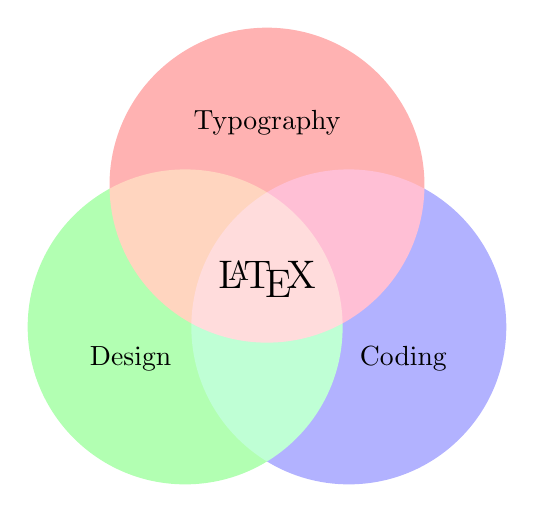
\begin{tikzpicture}
		\begin{scope}[blend group=soft light]
			\fill[red!30!white]   ( 90:1.2) circle (2);
			\fill[green!30!white] (210:1.2) circle (2);
			\fill[blue!30!white]  (330:1.2) circle (2);
		\end{scope}
		\node at ( 90:2) 	{Typography};
		\node at (210:2)  	{Design};
		\node at (330:2) {Coding};
		\node [font=\Large] {\LaTeX};
	\end{tikzpicture}
	\caption{Venn diagram TIKZ seg\'its\'egv\'evel}
\end{figure}

